\documentclass[a4paper,11pt]{report}

\usepackage{graphicx}
\usepackage{url}
\def\UrlFont{\rmfamily}
\usepackage{algorithm}
\usepackage[noend]{algorithmic}
\usepackage{amsthm}
\usepackage{multicol}
\usepackage{footmisc}
\usepackage{times} % use Times Font instead of Computer Modern
%\usepackage{epsfig} % for \psfig{file=sample.eps,width=3cm}
%\usepackage{epsf} % for \epsfile{file=sample.eps,scale=0.6}
%\usepackage{epsbox} % for \epsfile{file=sample.eps,scale=0.6}

%% dvipdfm (dvi->pdf)
% \usepackage[dvipdfm]{color,graphicx}
%% dvipdfm PDF
% \usepackage[dvipdfm,bookmarks=true,bookmarksnumbered=true,bookmarkstype=toc]{hyperref}
%% dvipdfm 
%% http://hamilcar.phys.kyushu-u.ac.jp/~hirata/dvipdfm/


\setcounter{tocdepth}{3}
\setcounter{page}{-1}

\setlength{\oddsidemargin}{0.1in}
\setlength{\evensidemargin}{0.1in} 
\setlength{\topmargin}{0in}
\setlength{\textwidth}{6in} 
% \setlength{\textheight}{10.1in}
\setlength{\parskip}{0em}
\setlength{\topsep}{0em}

\newcommand{\zu}[1]{{\gt \bf \ref{#1}}}

\usepackage{src/sie-jp-sjis}

\title{Aggregate Nearest Neighborhood Queries In Euclidean Space}
\author{Hayata Takagi\\ (Master's Program in Computer Science)}
\degree{}
\advisor{Advised by Hiroyuki Kitagawa}
\majorfield{Submitted to the Graduate School of Systems and Information Engineering}
\programfield{in Partial Fulfillment of the Requirements for the Degree of Master of Engineering at the University of Tsukuba}
\yearandmonth{March 2021}


\newtheoremstyle{mytheoremstyle} % name
    {0.7em}                      % Space above
    {0.7em}                      % Space below
    {\itshape}                   % Body font
    {}                           % Indent amount
    {\bfseries}                  % Theorem head font
    {.}                          % Punctuation after theorem head
    {.5em}                       % Space after theorem head
    {}                           % Theorem head spec (can be left empty, meaning ‘normal’)

\theoremstyle{mytheoremstyle}
\newtheorem{definition}{Definition}
\newtheorem{theorem}{Theorem}

\begin{document}
\maketitle
\thispagestyle{empty}
\newpage

\thispagestyle{empty}
\vspace*{20pt plus 1fil}
\parindent=1em
\noindent

\begin{center}
    \textbf{Abstract}
\end{center}
\vspace{0.2in}

Efficiency of finding nearest clusters is a principal factor in query processing and data mining, and this can be applied to location information services and services using point of interests (POI). However, no research is currently aimed at finding the nearest cluster of multiple query points. In this paper, we propose Aggregate Nearest Neighborhood Query (ANNH) for searching the nearest cluster of multiple queries with aggregation distance between multiple query points and clusters. Further, one disadvantage is that previous research represents clusters only by circles, and this does not address problems such as biased data points remaining in the cluster. Alternatively, we present a solution to this challenge in ANNH by evaluating cluster density by variance.

%%%%%
\par
\vspace{0pt plus 1fil}
\newpage

\pagenumbering{roman} % I, II, III, IV 
\tableofcontents
\listoffigures
%\listoftables

\pagebreak \setcounter{page}{1}
\pagenumbering{arabic} % 1,2,3


\chapter{Introduction}
Nearest Neighborhood query in the spatial database is an important problem in a variety of applications such as pattern recognition, POI (Point of Interest), and LBS (Location-based Services), and other Data Mining applications\cite{adeniyi2016automated}. A wide variety of topics involving nearest neighbor search have been studied, and more recently the Balanced Nearest Neighborhood Query (BNNH)\cite{BNNH} has been proposed. Compared to traditional nearest neighbor search, which finds the point closest to a given query point, BNNH finds the nearest cluster as a response. That is, BNNH query is a variation of the nearest neighbor query for grouped points. On the other hand, aggregate Nearest Neighbor Queries (ANN)\cite{ANN} receive multiple query points and return the nearest point to the query group based on a certain aggregate distance function. In these studies, a key problem is that it was not possible to search the nearest cluster for multiple queries. Based on this challenge, this paper concentrates on searching for the nearest cluster for multiple query points.

The following is an application example of this research. Fig. \ref{fig:example-sum} shows an example of searching for a restaurant. Suppose one travels from a starting place to an end place, and he/she wants to visit several restaurants with the shortest travel distance when he/she decides on the area to drop in. In this case, the departure point and the end point become the queries, and the restaurants are the data set. In the proposed method, the purpose is to find a dense data subset from which the total distance of the queries is minimum.

\begin{figure}
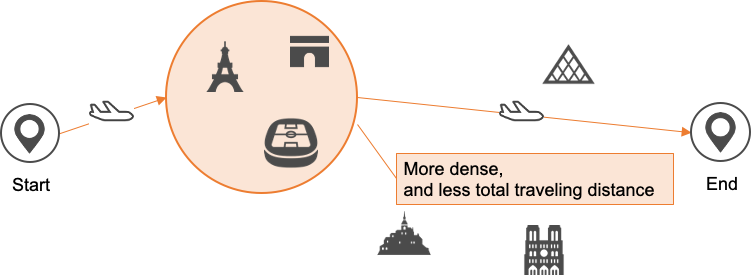
\includegraphics[width=\textwidth]{images/example-sum.png}
\caption{Example of minimizing the total distance} \label{fig:example-sum}
\end{figure}

Fig. \ref{fig:example-max} shows another example on determining a meeting place. Suppose the user wants to search for a place where plenty of activities are available and the members can gather easily. In this case, set of the locations of all users is the query, and the activity spots are the data set to be searched. The proposed method efficiently searches the cluster which the maximum distance from each user is less, and the density of activities is high. The cluster in Fig. \ref{fig:example-max2} does not satisfy the search request.
Although the density of cluster is almost the same as that of the cluster in Fig. \ref{fig:example-max}, it is not suitable as a meeting place because the maximum distance distance between each member of the query and the cluster is larger than the maximum value of the cluster in Fig. \ref{fig:example-max}.

To solve the above problem like in the example, we propose a new query processing problem of finding nearest neighborhood, named Aggregate Nearest Neighborhood Queries (ANNH).
ANNH searches for data points and finds clusters based on the proposed algorithm. ANNH calculates cluster scores using the evaluation function and finds a cluster which is denser and closer to the queries. ANNH evaluates the distance between multiple queries and a cluster using an aggregate distance function, and the cluster density using variance. The proposed ANNH is formally defined in Section \ref{section:annh}.

Major contributions of this paper are as follows.
\begin{itemize}
    \item  To define a general and realistic neighborhood query problem for multiple queries considering different neighborhood scale, we propose and formalize the Aggregated Nearest Neighbor Query (ANNH). ANNH uses smoothing parameters and aggregated distance functions to find a nearest cluster for multiple queries, responding to different user preferences between aggregate distance and scale.
  \item ANNH makes it possible to find more exact clusters by evaluating the cluster density by variance without fixing the cluster shape.
  \item To solve ANNH efficiently, we propose three methods: Point-based solution, Minimum bounding rectangle-based (MBR-based) solution and Grid-index-based solution. MBR-based solution utilizes the R-tree\cite{R-tree} structure to index points, and uses a best-distance methodology to filter unnecessary points. Grid-index-based solution is based on the grid structure\cite{BNNH}, which enables to retrieve k nearest neighbor points directly hence has better performance on ANNH query.
\end{itemize}

The rest of this paper is organized as follows. In Section \ref{section:related-works}, we introduce some related works. Section \ref{section:annh} describes the definition of Aggregated Nearest Neighbor Query (ANNH) and the proposed methods. The experimental results are discussed in Section \ref{section:experiments}. Section \ref{section:conclusion} concludes the paper.

\begin{figure}
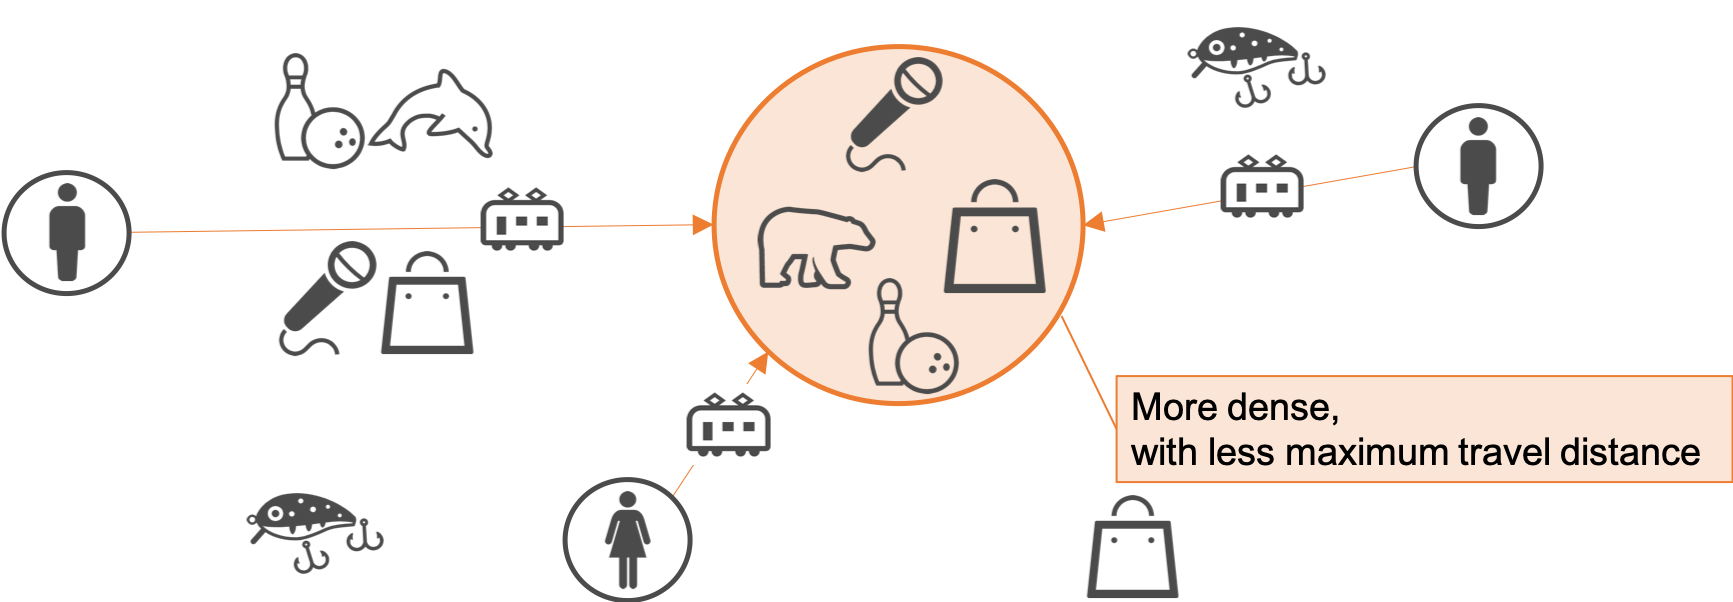
\includegraphics[width=\textwidth]{images/example-max.png}
\caption{An example of minimizing the maximum distance} \label{fig:example-max}
\end{figure}

\begin{figure}
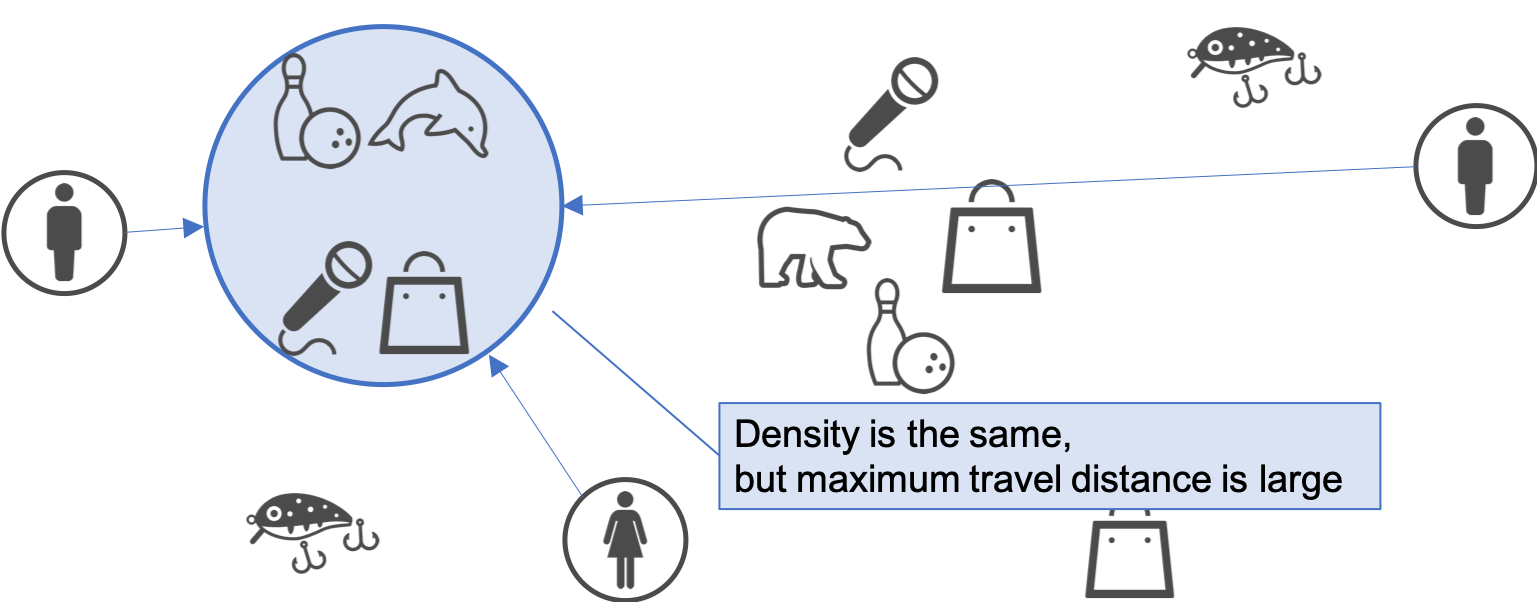
\includegraphics[width=\textwidth]{images/example-max2.png}
\caption{An example where maximum distance is not minimum} \label{fig:example-max2}
\end{figure}


\chapter{Related Work}
\label{section:related-works}

\section{Nearest neighbor query and best-first search on R-tree.}
In multiple fields including database management systems, data mining and information retrieval, a basic yet important problem is the (k) nearest neighbor query problem (NN, or kNN). Given a query point q and a point dataset $P$, NN returns the nearest point to $q$ from the dataset $P$. Research has been widely conducted focusing on solving the NN query with good performance, one of the most popular solutions proposed is R-tree based processing \cite{NN,cheung1998enhanced,hjaltason1999distance}. R-tree \cite{R-tree} is a spatial index that groups close points in space with the minimum bounding rectangle (MBR), and manages MBRs with a tree structure. Roussopoulos et al \cite{NN} first proposed an R-tree based method for processing the NN query with geographic information systems (GISs). Hjaltason et al \cite{hjaltason1999distance} proposed a best-first method with R-tree to solve the NN query. The best-first method searches the nearest neighbor in best first manner. This maintains a priority queue that contains the MBRs of R-tree with the order of minimum distance to query point $q$. In our research, we also propose the solutions with the best-first method to solve the ANNH query.

\section{Group version of nearest neighbor query.}
As real-life applications are dissatisfied with only evaluating the relationship between single points like the conventional NN query, many variants of the NN query have been studied. Papadias et al. developed aggregate nearest neighbor query (ANN) \cite{ANN} to retrieve points with the smallest aggregate distance to multiple query points in metric space. ANN inputs a group of query points Q and aims to find a nearest single point that has the smallest aggregate distance to Q. Thus, although ANNH and ANN are similar in that they receive multiple queries, the difference is that ANNH explores clusters whereas ANN explores points. Deng et al. \cite{GNG} proposed a group nearest group query (GNG), which is a spatial query returning a group of points. In GNG, the response group is evaluated based on the distance from the query for each point, whereas in ANNH, a set of points is regarded as a cluster, and the cluster density is also included in the evaluation. Besides evaluating the similarity in terms of the Euclidean distance function, Dong et al, \cite{dong2017grid} proposed an aggregate reverse rank query which uses an inner product function to evaluating the similarity between a point and a group of points in the spatial algorithm. Nearest neighborhood search (NNH) \cite{NNH} extends the NN query and for query point q returns the nearest cluster which is a a circle with fixed radius $\rho$. Because the radius is fixed, it is impossible to
always find the circle containing k points. The BNNH \cite{BNNH} extends NNH so that the radius can be changed to guarantee k points found, and the balance between the cluster size and the distance from the query point is considered using smooth parameters. While BNNH is given a single query point and judges clusters density by the radius of the circle, ANNH is given multiple query points and judges clusters density by the variance, so ANNH can find more dense clusters.

\chapter{Aggregate Nearest Neighborhood Queries}
\label{section:annh}
ANN \cite {ANN} takes multiple query points as input and outputs a single point. BNNH \cite{BNNH} takes a single point as input and clusters as output. ANNH realizes a combination of multiple queries for input and a cluster of nearest neighbors for query, which is a combination that cannot be searched in these previous studies.
In BNNH, a cluster was defined as a circle, and the density was defined as the radius of the circle. This requires a calculation to form a circle and presents a problem in that it is not possible to detect bias in the data inside a cluster. ANNH does not limit the shape of a cluster to a circle, evaluates the degree of congestion based on the variance within the cluster, thereby achieving a reduction in the amount of computation and searching for a denser cluster.

The notaions used in this paper are shown in Table \ref{tab:var}. Given a query $Q$, a cluster size $k$, and balancing parameters $\alpha$ and $\beta$, ANNH search is to find the cluster closest to the given query. ANNH are formally defined as follows:

\begin{table}
  \begin{center}
  \caption{Notations and symbols}
    \begin{tabular}{|l|l|} \hline
      Symbols & Description \\ \hline \hline
      $p, P$ & point, point set \\ \hline
      $q, Q$ & query point, query group \\ \hline
      $C, V_C$ & cluster, variance of cluster \\ \hline
      $O_C$ & cluster centroid \\ \hline
      $dist(p,q)$ & euclidean distance between $p$ to $q$ \\ \hline
      $f(p, C)$  & aggregation distance between point $p$ and cluster $C$ \\ \hline
      $\alpha$, $\beta$ & user preference parameter \\ \hline
      $k$ & response cluster size \\ \hline
      $\Delta(C,Q)$ & the evaluation function of $C$ and $Q$ \\ \hline
      $MBR$ & minimum bounding rectangle in a R-tree \\ \hline
      $n$ & cells number in location-base index \\ \hline
    \end{tabular}
    \label{tab:var}
  \end{center}
\end{table}

\begin{definition}
(Aggregate Nearest Neighborhood Queries, ANNH). Given a set of points P, a query group Q, a positive value $k$ and a user-defined smoothing parameter $\alpha$ and $\beta$. ANNH returns the neighborhood cluster C including k points, and C holds the minimum value of $\Delta(C, Q)$.
\end{definition}

The neighborhood is defined as a cluster as follows.

\begin{definition}
Given k, a neighborhood C is defined as a cluster including at least k points in the metric space.
\end{definition}

$V_C$ denotes the variance of C. The evaluation function $\Delta(.)$ used in ANNH is as follows, which is a evaluation function modified from the one proposed in BNNH\cite{BNNH}. The function $f(.)$ calculates the aggregation distance, which is described in detail in Section \ref{subsection:aggregate-distance}.

\begin{equation}
\label{equ:f-delta}
\Delta(C,Q) = \alpha \cdot f(O_C, Q) + \beta \cdot V_C\ \
\end{equation}

By changing the values of the smoothing parameters $\alpha$ and $\beta$ of Equation (\ref{equ:f-delta}), the user's preference can be reflected. For example, if $\alpha > \beta$, it is preferable that the cluster position is closer, and if $\alpha < \beta$, then it is preferable that the cluster density is higher, and in the case of $\alpha = \beta $, this indicates that the position and the density of the cluster are equally important. Fig. \ref{fig:example-delta} illustrates three clusters $C_1$, $C_2$ and $C_3$. In this example, $C_2$ is the answer because the cluster has the highest density and is closest to the query. In the comparison of $C_1$ and $C_3$, we cannot easily determine which is better, because $C_1$ is closer but $C_3$ is denser. Even in such case, we determine which is better by the evaluation function $\Delta(.)$.

\begin{figure}
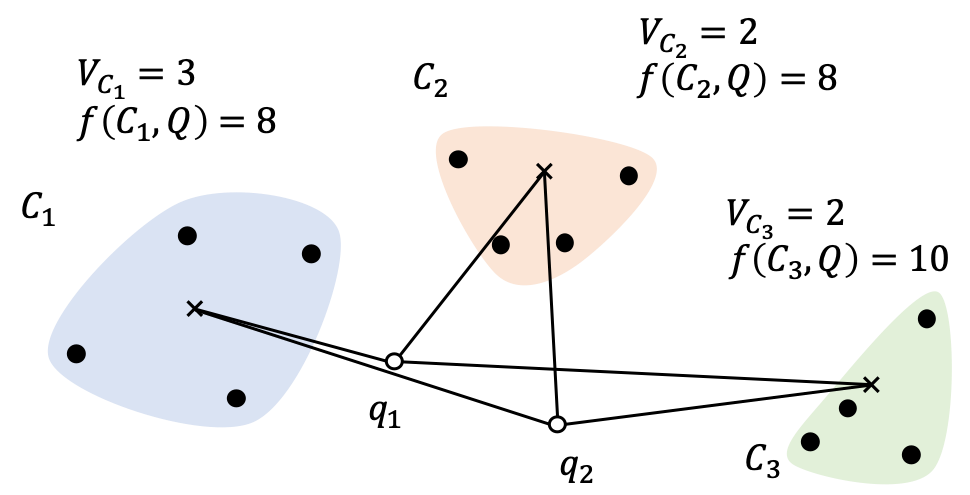
\includegraphics[width=\textwidth]{images/example-delta.png}
\caption{Relationship between cluster distance and density} \label{fig:example-delta}
\end{figure}


\section{Aggregation distance}
\label{subsection:aggregate-distance}
With multiple queries, it is necessary to define the nearest neighbor between a query group $Q$ and a point $p$. In this study, \textbf{sum} and \textbf{maximum} are taken as the nearest indices.

\section{Aggregate nearest neighborhood of sum.}
The cluster that minimizes the total distance from each query to the cluster is defined as the nearest neighborhood. As in the example shown in Fig. \ref{fig:example-sum}, the user can solve the problem of minimizing the traveling distance by setting the route point as a query itself. The equation for calculating the sum aggregation distance between a point $p$ and a query $Q$ is as follows.

\begin{equation}
\label{equ:f-sum}
f_{sum}(p,Q) = \sum_{i=1}^{n} dist(p,q_i)
\end{equation}

\section{Aggregate nearest neighborhood of maximum.}

The cluster in which the maximum value of the distance from each query to the cluster, is the least, is defined as the nearest neighborhood. As shown in Fig. \ref{fig:example-max}, the problem of selecting the waypoint when determining the meeting place at the user's location can be solved. The equation for calculating the max aggregation distance between a point $p$ and a query $Q$ is as follows.

\begin{equation}
\label{equ:f-max}
f_{max}(p,Q) = max_{i=1}^{n} dist(p,q_i)
\end{equation}

\section{Evaluation of Cluster Density}
The cluster density is represented by the intracluster variance $V$. When the centroid of the cluster $C$ formed by the points $p_1, \cdots p_n$ is $O_C$, the equation for calculating the variance of $C$ is shown below.

\begin{equation}
\label{equ:w}
V_C = \frac{1}{|C|} \sum_{i=1}^{n} \{dist(p_i, O_C)\}^2 
\end{equation}

\section{Estimating the Filtering Bound}
\label{subsection:filtering}
Creating the nearest neighbor cluster for every the data point $p$ and calculating the value of $\Delta(.)$ are very inefficient. To improve efficiency, filtering is performed before calculating the k-nearest neighborhood of the point $p$.

By dividing both sides of the evaluation formula by $\alpha +\beta$, we obtain the following formula.

\begin{equation}
\label{equ:filter-1}
\frac{\Delta(C,Q)}{\alpha+\beta} = \frac{\alpha}{\alpha+\beta} \cdot f(O_C, Q) + \frac{\beta}{\alpha+\beta} \cdot V_C\ \
\end{equation}

Since $\frac{1}{\alpha+\beta}$ is constant irrespective of the query or data set, the problem of $\frac{\Delta(C,Q)}{\alpha+\beta}$ is considered to be equivalent to $\Delta(C,Q)$. Hereafter, $\frac{\Delta(C,Q)}{\alpha+\beta}$ is expressed as $\Delta'(C,Q)$.

When $\alpha < \beta$, constant terms including $\alpha$ and $\beta$ are as follows.
\begin{equation}
\label{equ:filter-alpha-beta}
\frac{\beta}{\alpha} > 1
\end{equation}

Using Equation (\ref{equ:filter-alpha-beta}), Equation (\ref{equ:filter-1}) is transformed as follows.

$$\Delta'(C,Q) = \frac{\alpha}{\alpha+\beta} \cdot f(O_C, Q) + \frac{\beta}{\alpha+\beta} \cdot V_C$$

$$\frac{\alpha+\beta}{\alpha} \cdot \Delta'(C,Q) = f(O_C, Q) + \frac{\beta}{\alpha} \cdot V_C$$

\begin{equation}
\label{equ:filter-2}
\frac{\alpha+\beta}{\alpha} \cdot \Delta'(C,Q) > f(O_C, Q) + V_C
\end{equation}

The following theorem of filtering can be derived from Equation (\ref{equ:filter-2}).

\begin{theorem}
Given a query group $Q$ and a cluster $C$. Any cluster containing point p cannot be a better solution than $C$ if
$f(p,Q) > \frac{\alpha + \beta}{min(\alpha, \beta)} \cdot \Delta(C,Q)$.
\end{theorem}

\begin{proof}
Assume that a query group $Q$ is given, $C_1$ is the current best cluster, and that a specific point $p$ does not belong to $C_1$. Assume also that $\alpha < \beta$. According to Equation (\ref{equ:filter-2}), if we create an arbitrary cluster $C_2$ with $p$ and other points, then
$$f(p,Q) \leq f(O_{C_2}, Q) + V_{C_2} < \frac{\alpha+\beta}{\alpha} \cdot \Delta(C_2,Q) $$
Therefore, if $p$ locates further than the bound $\frac{\alpha + \beta}{\alpha} \cdot  \Delta(C_1,Q)$ which created by the current best cluster $C_1$ (i.e., $f(p,Q) > \Delta(C_1,Q)$), we can infer that $\Delta(C_1, Q) < \Delta(C_2, Q)$. Hence, any cluster that contains $p$ will not better than $C_1$.
\end{proof}
From the theorem, whenever we find a current best cluster $C$, a point $p$ can be safely filtered if it locates out of the bound.

\section{Point-based solution}

A method for searching for a cluster using Equation (\ref{equ:f-delta}) is described below. The first is a simple point-based search method. It finds the nearest $k-1$ points for each dataset point and computes the cluster. If the evaluation value of this cluster is better than the nearest cluster found so far, then it is updated. It is necessary to perform filtering as described in Section \ref{subsection:filtering} before creating the cluster. The pseudo code of the point-based method is shown in Algorithm \ref{alg:point}. We create cluster $C_t$ using the nearest $k-1$ points for a point having the aggregate distance less than the current best bound (Line 4-6). If the $\Delta(.)$ value of $C_t$ is less than the current best bound, $C_t$ is set to current best solution and the bound is updated to the aggregate distance on $C_t$ (Line 7-9).

\begin{algorithm}                      
\caption{Point-based Solution}         
\label{alg:point}
\begin{algorithmic}[1]                  
\renewcommand{\algorithmicrequire}{\textbf{Input:}}
\renewcommand{\algorithmicensure}{\textbf{Output:}}
\REQUIRE $P,Q,k,\alpha, \beta$
\ENSURE $C$
\STATE $bound \xleftarrow{} \infty$
\STATE $C \xleftarrow{} \emptyset$
\FOR{$each\ p_i \in P$}
\IF{$f(p_i,Q)<bound$}
\STATE $pSet \xleftarrow{} p_i$ and its $k-1$ nearest points
\STATE $C_t \xleftarrow{}$ create Cluster with $pSet$
\IF{$\Delta(C_t,Q)<bound$}
\STATE $C \xleftarrow{} C_t$
\STATE update $bound$ with $\Delta(C_t,Q)$
\ENDIF
\ENDIF
\ENDFOR
\RETURN $C$
\end{algorithmic}
\end{algorithm}

\section{MBR-based solution}
In the point-based method, filtering is performed on the data points one by one. If filtering is performed on blocks of points such as $MBR$ of the R-tree, filtering can be more efficient, and a reduction in the amount of calculation can be expected. In MBR-based solution, the dataset is indexed in a R-tree, and $Q$ is also bounded by their MBR. By filtering at a distance of $Q$ from each node, filtering can be performed immediately. Figure \ref{fig:solution-mbr} shows the relationship between the MBR of a query $Q$ and MBRs of clusters $N_1$ and $N_2$. For example, if the current bound is 4, ANNH explore $N_1$ because its minimum distance to the MBR of the query MBR is less than the bound. However, $N_2$ can be pruned because its minimum distance to the MBR of the query is greater than bound. Algorithm \ref{alg:mbr} shows the pseudo-code of the method using the R-tree. We initialize the bound with the nearest point of $Q$ (Line 1-4). We prune the MBRs if the minimum distance between the MBRs and the query $Q$ is larger than the bound (Line 8). We calculate the $\Delta(.)$ value for a point in the leaf nodes and update the result and the bound if it is less than the current value (Line 14-18).

\begin{figure}
\begin{center}
    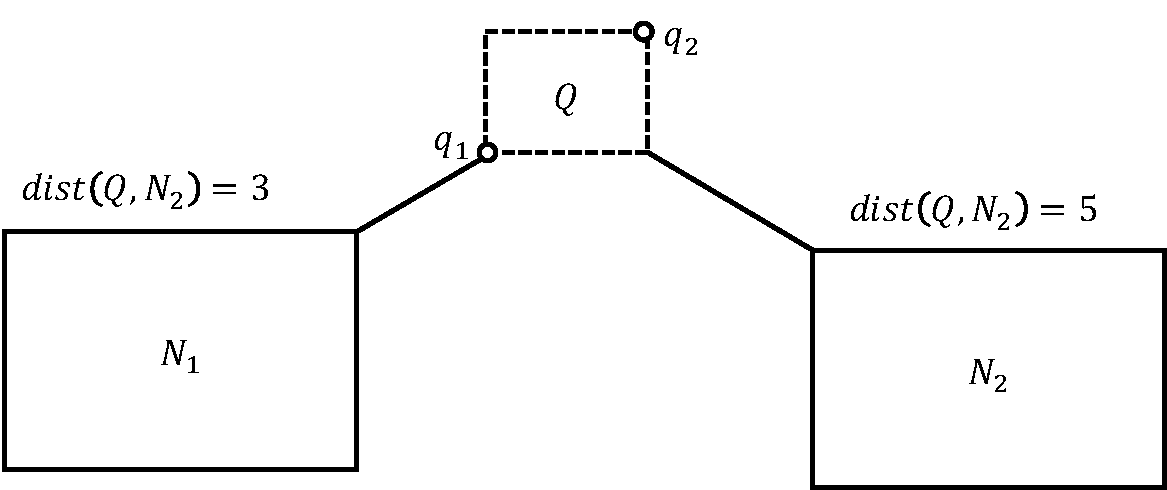
\includegraphics[width=0.8\textwidth]{images/solution-mbr.pdf}
\end{center}
\caption{MBR-based solution} \label{fig:solution-mbr}
\end{figure}

\begin{algorithm}
\caption{MBR-based solution}         
\label{alg:mbr}
\begin{algorithmic}[1]                  
\renewcommand{\algorithmicrequire}{\textbf{Input:}}
\renewcommand{\algorithmicensure}{\textbf{Output:}}
\REQUIRE $P,Q,k,\alpha, \beta$
\ENSURE $C$
\STATE $p_a \xleftarrow[]{}$ the nearest point to $Q$ from $P$.
\STATE $pSet \xleftarrow{} p_a$ and its $k-1$ nearest points
\STATE $C \xleftarrow[]{}$ create Cluster with pSet
\STATE $bound \xleftarrow[]{} $calculate the filter condition with $\Delta(C,Q)$
\STATE $heep \xleftarrow[]{} Rtree.root$
\WHILE{$heap$ is not empty}
\STATE $E \xleftarrow[]{}heap.front()$
\IF{$mindit(E,Q)<bound$}
\IF{$E$ is none-leaf node}
\STATE $heap \cap E.children$
\ENDIF
\IF{$E$ is leaf node}
\FOR{each $p \in E$}
\IF{$dist(p_i, Q) < bound$}
\STATE $pSet \xleftarrow{} p_i$ and its $k-1$ nearest points
\STATE $C_t \xleftarrow{}$ create Cluster with $pSet$
\IF{$\Delta(C_t,Q)<\Delta(C,Q)$}
\STATE $C \xleftarrow{} C_t$
\STATE update $bound$ with $\Delta(C_t,Q)$
\ENDIF
\ENDIF
\ENDFOR
\ENDIF
\ENDIF
\ENDWHILE
\RETURN $C$
\end{algorithmic}
\end{algorithm}

\section{Grid-index-based solution}

We notice that in the proposed point-base and group-base solutions, the most time-consuming task is to find the kNN points for a specific point (Line 5 in Algorithm \ref{alg:point} and Line 14 in Algorithm \ref{alg:mbr}). This can be avoided by reducing the number of clusters created by filtering. It has also been reported that, in NN search filtering, if a search is performed near a query point, the filtering bound is reduced and the amount of filtering is increased \cite{BNNH}. From this, the data set is arranged on the grid in the two-dimensional space, as in the previous studies \cite{BNNH,weber1998quantitative,mouratidis2006continuous,yu2005monitoring,mouratidis2005conceptual,xiong2005sea}. Figure \ref{fig:solution-grid} shows an example where there is one query point (or the center of the query MBR). The cell in which the query $q'$ exists can be specified, and cells around it can be searched. Thus, the search can be performed efficiently. The bound is represented by a dotted-line circle in the Figure \ref{fig:solution-grid}, and only the cells within the dotted-line circle need to be searched. In ANNH, the starting point of the cell searched in the case of multiple queries is the centroid of the query group. Algorithm \ref{alg:grid} shows a pseudo-code of the grid-index-based method. The bound is initialized to the evaluation value for the nearest point of $Q$ (Line 1-4). Cells are expanded from around the query $Q$ (Line 5). We create the clusters using the points nearest to $Q$ in the cells (Line 7-9). The clusters are created from the points in these cells and the corresponding $\Delta(.)$ are calculated. The current best solution and the bound are updated the bound is better than the current one (Line 10-12). 

\begin{figure}
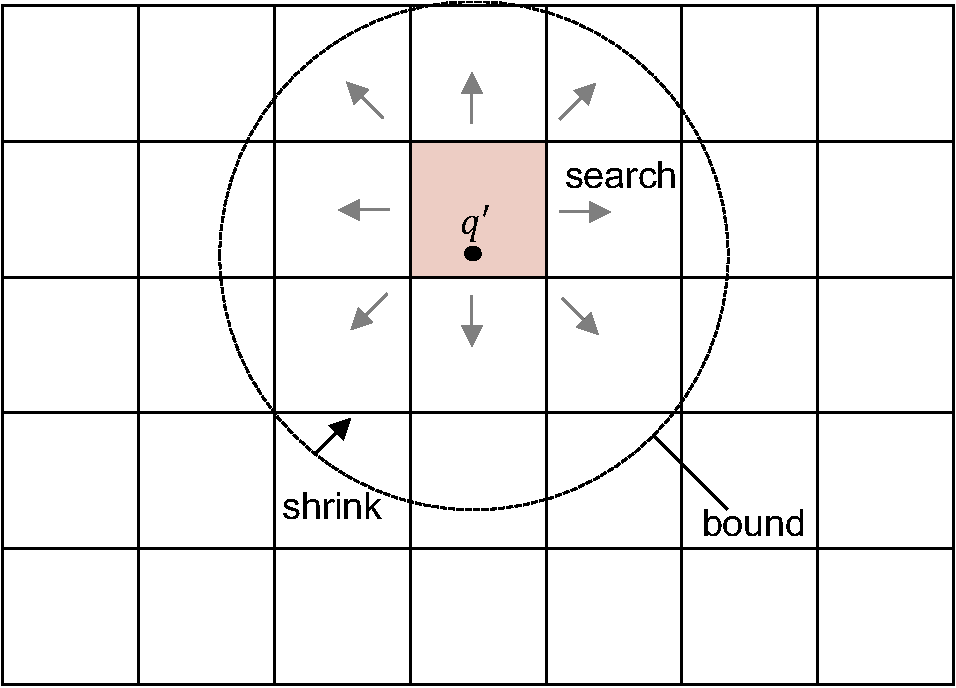
\includegraphics[width=\textwidth]{images/solution-grid.pdf}
\caption{Grid-index-based solution} \label{fig:solution-grid}
\end{figure}


\begin{algorithm}                      
\caption{Grid-index-based solution}         
\label{alg:grid}
\begin{algorithmic}[1]                  
\renewcommand{\algorithmicrequire}{\textbf{Input:}}
\renewcommand{\algorithmicensure}{\textbf{Output:}}
\REQUIRE $P,Q,k,\alpha, \beta$
\ENSURE $C$
\STATE $p_a \xleftarrow[]{}$ the nearest point to $Q$ from $P$.
\STATE $pSet \xleftarrow{} p_a$ and its $k-1$ nearest points
\STATE $C \xleftarrow[]{}$ create Cluster with pSet
\STATE $bound \xleftarrow[]{} $calculate the filter condition with $\Delta(C,Q)$
\STATE $nextCells \xleftarrow[]{} $ get surround cells of $Q$
\WHILE{nextCells locate in $bound$}
\STATE $pNext \xleftarrow[]{}$ retrieve nearest point to $Q$ from $nextCells$
\STATE $pSet \xleftarrow[]{} pNext$ and its $k-1$ nearest points
\STATE $C_t \xleftarrow{}$ create Cluster with $pSet$
\IF{$\Delta(C_t,Q)<\Delta(C,Q)$}
\STATE $C \xleftarrow{} C_t$
\STATE update $bound$ with $\Delta(C_t,Q)$
\ENDIF
\STATE $nextCells \xleftarrow[]{} $ the next round of cells
\ENDWHILE
\RETURN $C$
\end{algorithmic}
\end{algorithm}

\section{Quadtree-based solution}
We can now explore from the neighborhood of the query by grid, but grid cannot deal with the bias of the dataset because grid divide the dataset uniformly. For example, when a dataset is placed on a grid cell far away from the query, as shown in Figures \ref{fig:solution-quadTree1}, useless searches will occur. To solve this problem, we introduce quadtree \cite{finkel1974quad}, which has been shown to be effective in NN problems by Shin et al.\cite{shin2019investigation}, and we propose a search method for quadtree to solve the ANNH queries efficiently.

Figures \ref{fig:solution-quadTree2} shows an example of our proposed quadtree. In this case, the threshold is 2, the red dot is the center of gravity of the query, the black dot is the dataset, the dotted line is the grid, and the blue line is the boundary of the nodes in the quadtree. We use grids as an adjunct to quadtree, and a grid has the address of the node to which it belongs. For example, $g_1$ belongs to node $N_1$, so it has an address of $N_1$, and similarly $g_2$ has an address of $N_2$. Also, each node has a flag called $is_visited$, which indicates whether the node has been explored or not.

Algorithm \ref{alg:quadtree} shows a pseudo-code of the quadtree-based method. The bound is initialized to the evaluation value for the nearest point of $Q$ (Line 1-4). Cells are expanded from around the query $Q$ (Line 5). If there are points in the visited cell, the point closest to the centroid of the query in the cell is used as pNext, otherwise, the point closest to the centroid of the query in node to which the cell belongs is used as pNext (Line 7-12). We create the clusters using pNext from the previous step and calculate $\Delta(.)$. If $\Delta(.)$ value is better than the current best cluster, update the best cluster and the bound. (Line 13-17). Then, set the $is_visited$ flag of the visited node to true (Line 18). We repeat this steps for every cell in the non-visited node in the bound (Line 19).

\begin{figure}
    \begin{center}
        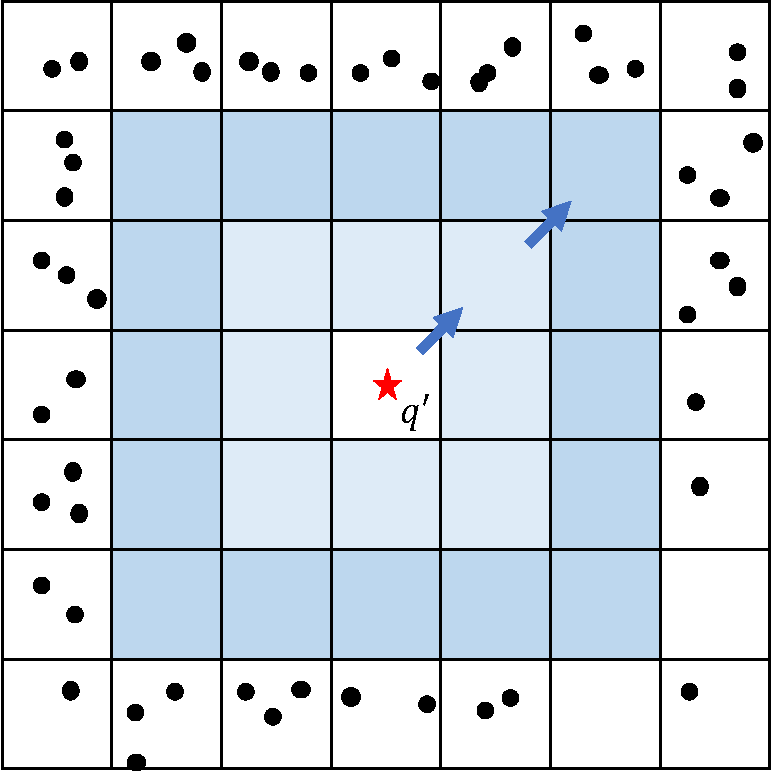
\includegraphics[width=0.6\textwidth]{images/solution-QuadTree1.pdf}
        \caption{An example of Grid-index-based solution that occur unnecessary search} \label{fig:solution-quadTree1}
    \end{center}
\end{figure}

\begin{figure}
    \begin{center}
        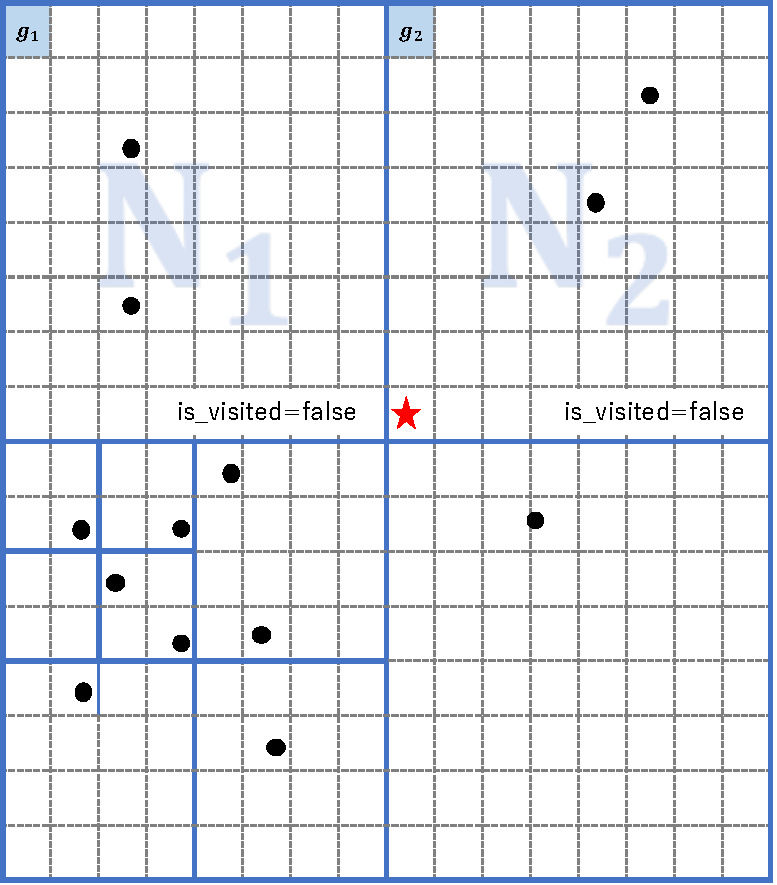
\includegraphics[width=0.6\textwidth]{images/solution-QuadTree2.pdf}
        \caption{Quadtree-based solution} \label{fig:solution-quadTree2}
    \end{center}
\end{figure}

\begin{algorithm}                      
\caption{Quadtree-based solution}         
\label{alg:quadtree}
\begin{algorithmic}[1]                  
\renewcommand{\algorithmicrequire}{\textbf{Input:}}
\renewcommand{\algorithmicensure}{\textbf{Output:}}
\REQUIRE $P,Q,k,\alpha, \beta$
\ENSURE $C$
\STATE $p_a \xleftarrow[]{}$ the nearest point to $Q$ from $P$.
\STATE $pSet \xleftarrow{} p_a$ and its $k-1$ nearest points
\STATE $C \xleftarrow[]{}$ create Cluster with pSet
\STATE $bound \xleftarrow[]{} $calculate the filter condition with $\Delta(C,Q)$
\STATE $nextCells \xleftarrow[]{} $ get surround cells of $Q$
\WHILE{nextCells locate in $bound$}
\FOR{\textbf{each} $cell \in nextCells$}
\STATE $node \xleftarrow[]{}$ the node where $cell$ is located
\IF{$cell$ has points}
\STATE $pNext \xleftarrow[]{}$ retrieve nearest point to $Q$ from $cell$
\ELSE
\STATE $pNext \xleftarrow[]{}$ retrieve nearest point to $Q$ from $node$
\ENDIF
\STATE $pSet \xleftarrow[]{} pNext$ and its $k-1$ nearest points
\STATE $C_t \xleftarrow{}$ create Cluster with $pSet$
\IF{$\Delta(C_t,Q)<\Delta(C,Q)$}
\STATE $C \xleftarrow{} C_t$
\STATE update $bound$ with $\Delta(C_t,Q)$
\ENDIF
\STATE $node$'s is\_visited $\xleftarrow[]{}$ $true$
\ENDFOR
\STATE $nextCells \xleftarrow[]{} $ cells located in non-visited nodes arround the query
\ENDWHILE
\RETURN $C$
\end{algorithmic}
\end{algorithm}

\chapter{Experiments}
\label{section:experiments}

We conducted a sufficient amount of experiments to verify the efficiency of our proposal. All algorithms for the solutions presented were implemented in C++. The experiments were conducted on a Mac operating system with the specifications as follows: macOS 10.15.5 (19F101), with a 3.2 GHz 6-Core Intel Core i7 processor, memory of 36 GB 2667 MHz DDR4.

\section{Datasets}
We performed experiments using geographic datasets and synthetic data sets. The geographic datasets are NE (123,593 points) and CAS (196,902 points) obtained from the US Census TIGER Project \cite{chorochronos}. For the synthetic data, a data set (10K - 100K points) based on uniform distribution is created and used.

\section{Parameters}
Query point is randomly selected from a dataset. The default result size $k$ is 50 and parameter $\alpha$ and $\beta$ are 0.5. The grid size for grid-index-based solution is 128, and the default grid size for the quadtree-based solution is 512. All results are reported as the sum processing time 100 times conducting ANNH queries. We set the quadtree threshold to 20 because preliminary experiments showed that it has no effect on the speed and the result cluster.

\section{Experimental results}

The result of changing the query size using NE dataset is shown in Figures \ref{fig:sum-querySize} and  \ref{fig:max-querySize}. The quadtree-based method is the fastest for the sum and the maximum aggregate distances, followed by the grid-index-based method. This is because the search is performed from the vicinity of queries in the grid-index-based method and the quadtree-based method, therefore the bound used for filtering is appropriately set early and the amount of filtering is large. In the grid-index-based method for the sum aggregate distance, the result becomes faster as the query size becomes larger. This is because the larger the number of queries, the more appropriately bound is set and the larger the amount of filtering is.
The quadtree-based method was about 10 times faster than the grid-index-based method. This is because the grid divides the dataset uniformly, which causes unnecessary searches for cells which have no points, while the quadtree has no node which has no points because it determines the size of a node based on the density of points in the node, which reduces unnecessary searches and speeds up.

\begin{figure}
    \begin{center}
        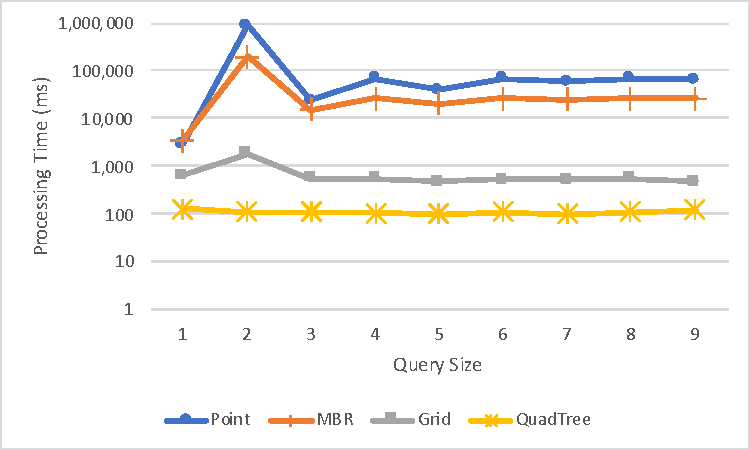
\includegraphics[width=0.8\textwidth]{src/images/NE-SUM-Q.pdf}
    \end{center}
    \caption{Running time versus query size.(Dataset: NE, Aggregation distance: SUM)}
    \label{fig:sum-querySize}
\end{figure}

\begin{figure}
    \begin{center}
        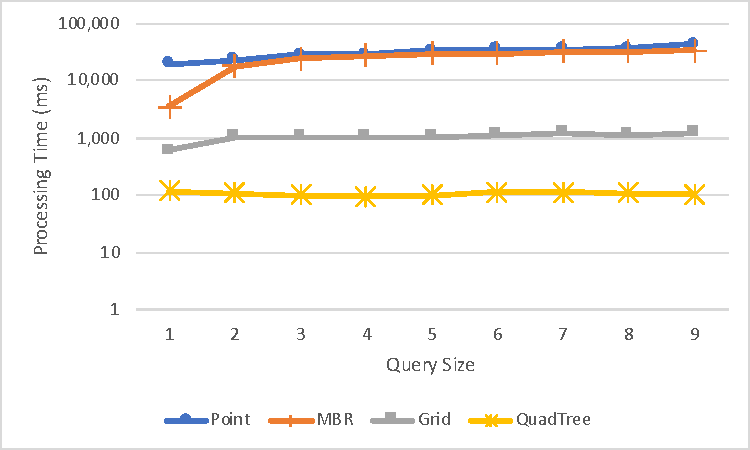
\includegraphics[width=0.8\textwidth]{src/images/NE-MAX-Q.pdf}
    \end{center}
    \caption{Running time versus query size.(Dataset: NE, Aggregation distance: MAX)}
    \label{fig:max-querySize}
\end{figure}

The result of changing the query size using CAS dataset is shown in Figures \ref{fig:sum-querySize-CAS} and  \ref{fig:max-querySize-CAS}. The results in CAS are same trend as the NE results.

\begin{figure}
    \begin{center}
        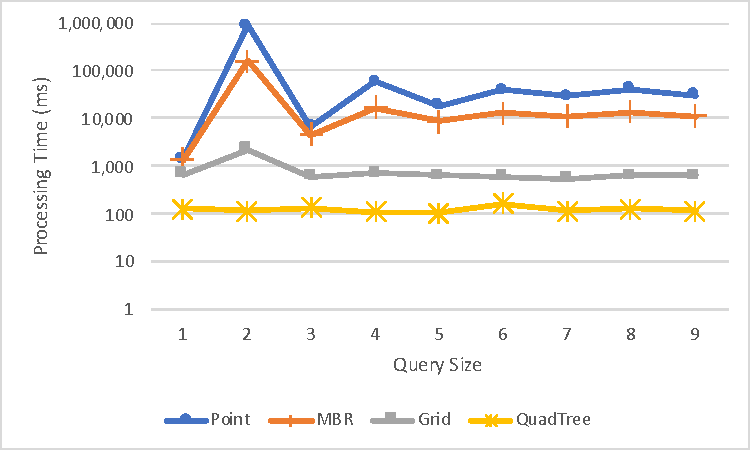
\includegraphics[width=0.8\textwidth]{src/images/CAS-SUM-Q.pdf}
    \end{center}
    \caption{Running time versus query size.(Dataset: CAS, Aggregation distance: SUM)}
    \label{fig:sum-querySize-CAS}
\end{figure}

\begin{figure}
    \begin{center}
        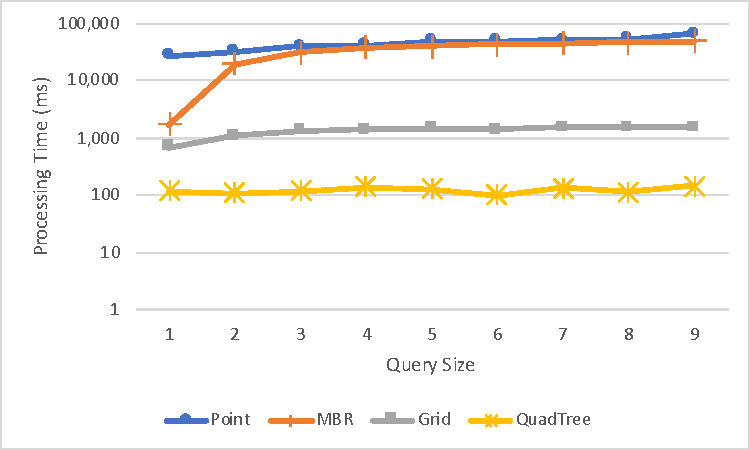
\includegraphics[width=0.8\textwidth]{src/images/CAS-MAX-Q.pdf}
    \end{center}
    \caption{Running time versus query size.(Dataset: CAS, Aggregation distance: MAX)}
    \label{fig:max-querySize-CAS}
\end{figure}

The result of changing the cluster size is shown in Figures \ref{fig:sum-clusterSize} and \ref{fig:max-clusterSize}. The quadtree-based method is the fastest for both aggregation distances.

\begin{figure}
    \begin{center}
        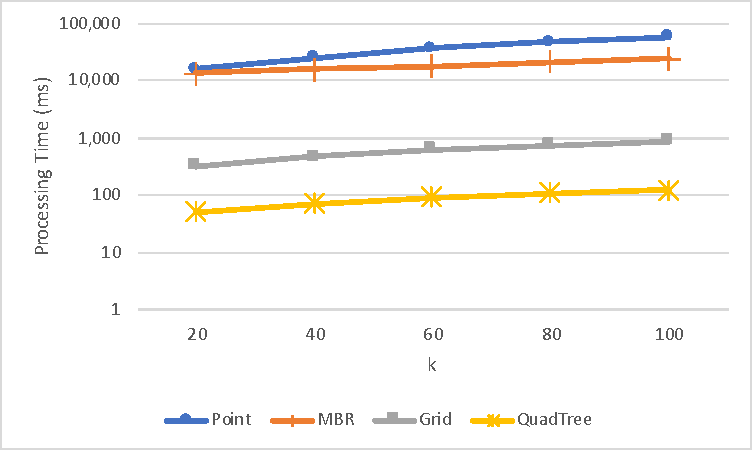
\includegraphics[width=0.8\textwidth]{src/images/NE-SUM-K.pdf}
    \end{center}
    \caption{Running time versus cluster size.(Dataset: NE, Aggregation distance: SUM)}
    \label{fig:sum-clusterSize}
\end{figure}

\begin{figure}
    \begin{center}
        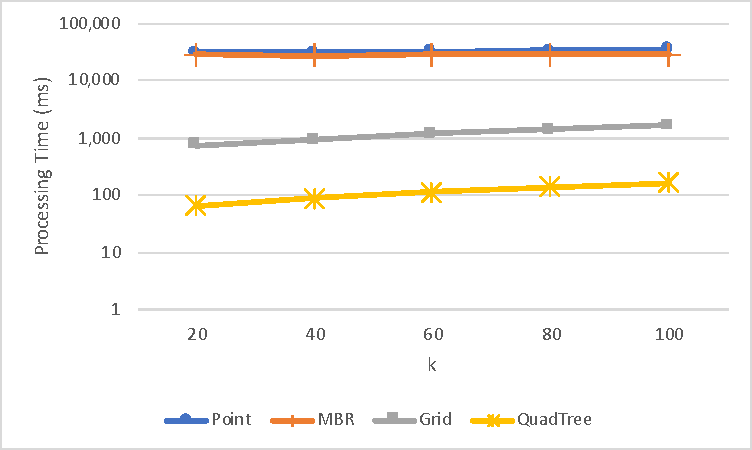
\includegraphics[width=0.8\textwidth]{src/images/NE-MAX-K.pdf}
    \end{center}
    \caption{Running time versus cluster size.(Dataset: NE, Aggregation distance: MAX)}
    \label{fig:max-clusterSize}
\end{figure}

The result of changing the cluster size using CAS dataset is shown in Figures \ref{fig:sum-clusterSize-CAS} and \ref{fig:max-clusterSize-CAS}. The results in CAS are same trend as the NE results.

\begin{figure}
    \begin{center}
        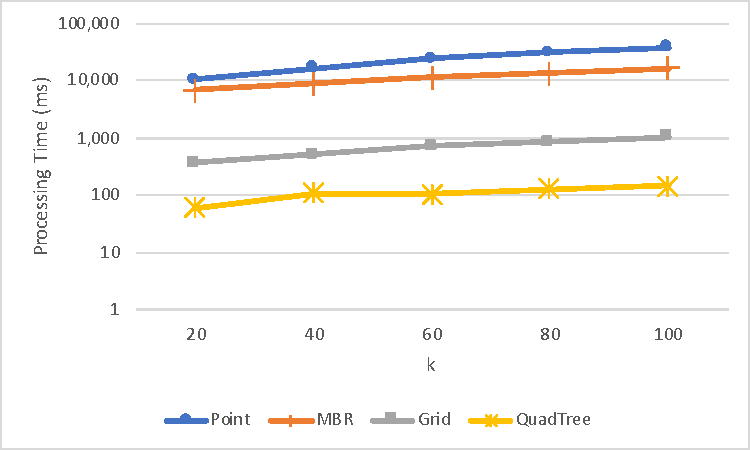
\includegraphics[width=0.8\textwidth]{src/images/CAS-SUM-K.pdf}
    \end{center}
    \caption{Running time versus cluster size.(Dataset: CAS, Aggregation distance: SUM)}
    \label{fig:sum-clusterSize-CAS}
\end{figure}

\begin{figure}
    \begin{center}
        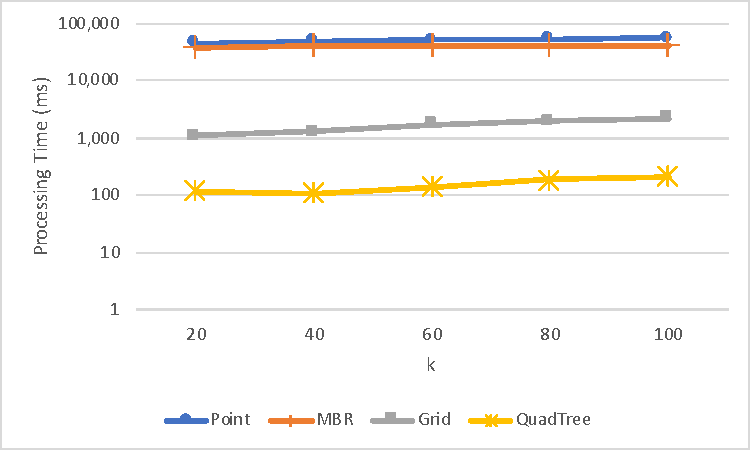
\includegraphics[width=0.8\textwidth]{src/images/CAS-MAX-K.pdf}
    \end{center}
    \caption{Running time versus cluster size.(Dataset: CAS, Aggregation distance: MAX)}
    \label{fig:max-clusterSize-CAS}
\end{figure}

The result of changing the data size is shown in Figure \ref{fig:sum-dataSize} and Figure \ref{fig:max-dataSize}. The processing time in grid-index-based method had a slower increasing trend than it in point-based method and mbr-based method. This is because the dataset is uniformly distributed, and there is a best cluster near the query.
For the aggregate distance SUM, the processing time in the quadtree-based method became faster as the data size increased within the range of the data size where we experimented, and the quadtree-based method became the fastest with a data size of 50,000. This does not mean that it becomes faster as the data size increases, but rather that the appropriate grid size for a quadtree depends on the data size, and for the default grid size for a quadtree of 512, points were placed on nodes more appropriately when the data size was 100,000 rather than 10,000. The same trend was observed for the aggregation distance MAX, where a data size of 100,000 was more appropriate than 10,000 for the grid size of 512 for a quadtree.

\begin{figure}
    \begin{center}
        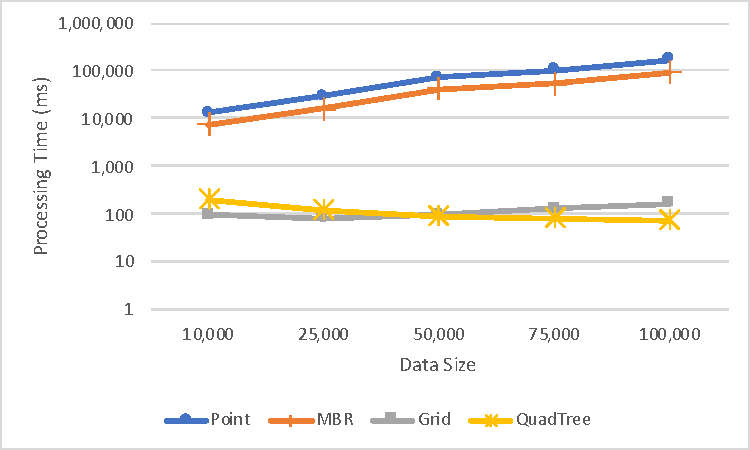
\includegraphics[width=0.8\textwidth]{src/images/UN-SUM.pdf}
    \end{center}
    \caption{Running time versus dataset size.(Dataset: UN, Aggregation distance: SUM)}
    \label{fig:sum-dataSize}
\end{figure}

\begin{figure}
    \begin{center}
        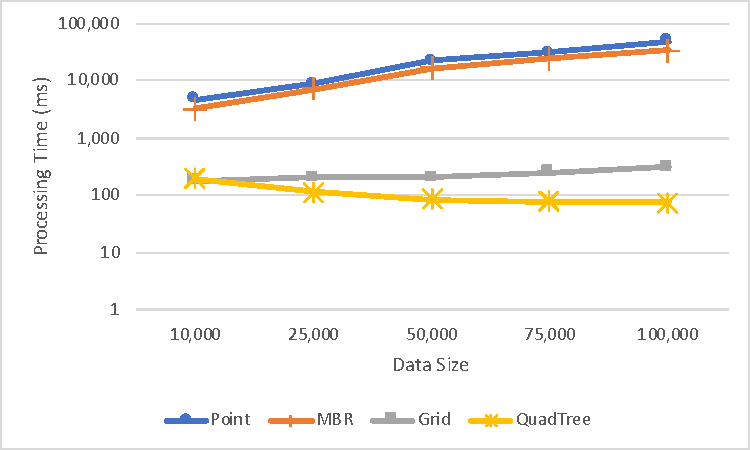
\includegraphics[width=0.8\textwidth]{src/images/UN-MAX.pdf}
    \end{center}
    \caption{Running time versus dataset size.(Dataset: UN, Aggregation distance: MAX)}
    \label{fig:max-dataSize}
\end{figure}

The result of changing the grid size is shown in Figure \ref{fig:sum-gridSize} and Figure \ref{fig:max-gridSize}. For both aggregate distances SUM and MAX, the quadtree-based method is faster than grid-index-based method when the grid size of quadtree is 256 and 512. It is assumed that when the size of the base grid for a quadtree was appropriate for the distribution of the dataset, the points are properly placed on the nodes and the search is fast.

\begin{figure}
    \begin{center}
        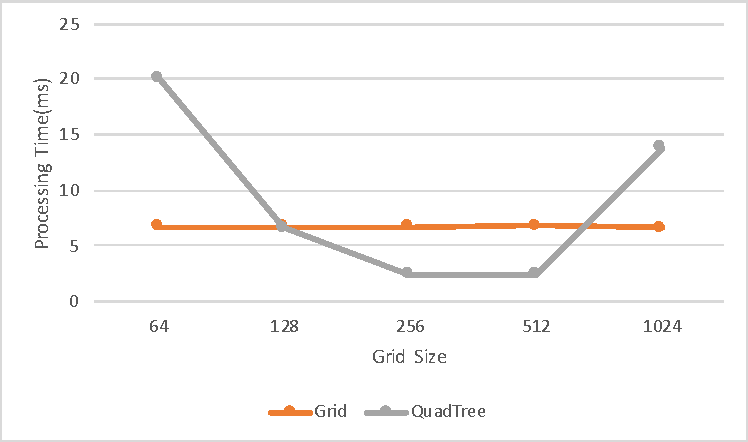
\includegraphics[width=0.8\textwidth]{src/images/CAS-SUM-GridSize.pdf}
    \end{center}
    \caption{Running time versus grid size.(Dataset: CAS, Aggregation distance: SUM)}
    \label{fig:sum-gridSize}
\end{figure}

\begin{figure}
    \begin{center}
        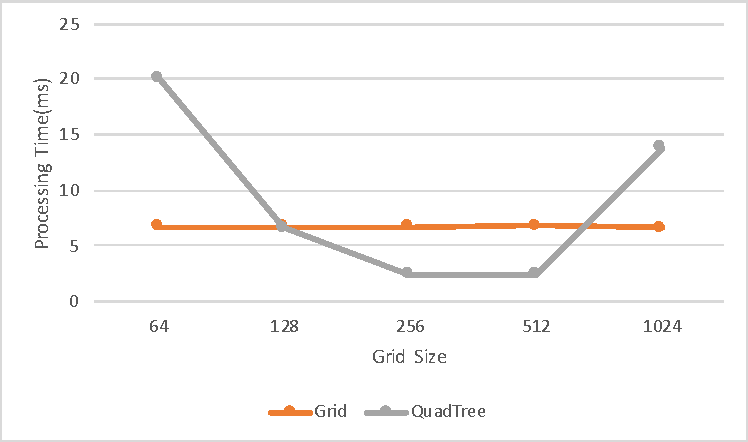
\includegraphics[width=0.8\textwidth]{src/images/CAS-SUM-GridSize.pdf}
    \end{center}
    \caption{Running time versus grid size.(Dataset: CAS, Aggregation distance: MAX)}
    \label{fig:max-gridSize}
\end{figure}

\chapter{Conclusion and future work}
\label{section:conclusion}

Finding the nearest cluster is an important issue in query processing and data mining. In previous research, it was not possible to search the nearest cluster of multiple queries. In this paper, the nearest neighbor cluster search of multiple queries was realized by defining the aggregation distance. We proposed four methods to search clusters, using point-based, MBR-based, grid-index-based and quadtree-based approaches. Experiments using both real data and synthetic data revealed that the method using a quadtree and a grid at all aggregation distances was the most efficient.

However, one drawback is that performance tends to decrease depending on the value of the smoothing parameter. Hence, our future work will now concentrate on solving this challenge.


\chapter*{Acknowledgements}
This work was supported by JSPS KAKENHI Grant Number JP19K12114.

\bibliographystyle{unsrt}
\bibliography{main}

\end{document}
